%========================================================================================
% LVC 2017 poster SpinTaylorF2 bounds
% Soham M 
%========================================================================================

\documentclass[final,hyperref={pdfpagelabels=false}, 11pt]{beamer}
\usepackage[orientation=portrait,size=a0,scale=1.17]{beamerposter} 
\usetheme{I6pd2} 
\usepackage[english]{babel} 
\usepackage{amsmath,amsthm,amssymb,latexsym} 
\usepackage[export]{adjustbox}
\makeatletter
\def\maketag@@@#1{\hbox{\m@th\normalfont\footnotesize#1}}
\makeatother

\usepackage{framed, color}
\definecolor{shadecolor}{rgb}{1, 0.8, 0.5}

\usepackage{booktabs} % Top and bottom rules for tables
\usepackage{ragged2e}
\graphicspath{{figures/}} % Location of the graphics files
\usepackage[utf8]{inputenc}
\usepackage{color}
\usecaptiontemplate{\footnotesize\structure{\insertcaptionname~\insertcaptionnumber:
}\insertcaption} % A fix for figure numbering

\setlength\abovecaptionskip{-20pt}
\usebackgroundtemplate{bg=white}

%========================================================================================
% TITLE SECTION 
%========================================================================================

\title{\huge \fontfamily{phv}\selectfont Probing astrophysical parameters of a
precessing binary using harmonics of SpinTaylorF2} % Poster title
\author{{\footnotesize{\fontfamily{qhv}\selectfont Soham
Mukherjee, K. Haris, K. Atmjeet, Archana Pai and \'E Chassande-Mottin}}} % Author(s)
\institute{\footnotesize{\fontfamily{qhv}\selectfont IISER Thiruvananthapuram, APC Paris}}% Institution(s)

\newcommand{\leftfoot}{\fontfamily{phv}\selectfont\footnotesize{LVC Meeting, Pasadena, March 2017}} % Left footer text
\newcommand{\rightfoot}{\fontfamily{phv}\selectfont\footnotesize{soham.m@iisertvm.ac.in}} % Right footer text

%========================================================================================
% BEGIN DOCUMENT 
%========================================================================================
\begin{document}
\addtobeamertemplate{block end}{}{\vspace*{1ex}} % White space under blocks
\begin{frame}[t] % The whole poster is enclosed in one beamer frame
\vskip1ex

%===========================================
\begin{columns}[b] % BEGIN SEC I
%===========================================
\begin{column}{.01\textwidth}\end{column} % Empty spacer column
\begin{column}{.97\textwidth} % central column with abstract text
\justifying
\small\textbf{Abstract}: 
We evaluate the contribution to the signal-to-noise ratio of the dominating
harmonics of \textit{SpinTaylorF2SingleSpin}---a single-spin, frequency
domain waveform model that incorporates the effects of spin-induced
precession. We show that the observation of specific harmonics can provide
direct evidence of precession. We also show that using the information from
two of the harmonics, we can infer the binary spin orientation and put bounds
on the spin-orbit parameters of the source.
\end{column} % End of central column
\begin{column}{.01\textwidth}\end{column} % Empty spacer column
%===========================================
\end{columns} % END SEC I
%===========================================

%===========================================
\begin{columns}[t] %BEGIN SEC II
%===========================================
\begin{column}{.01\textwidth}\end{column} % Empty spacer column

%===============================================================
\begin{column}{.35\textwidth} % BEGIN SEC II COL 1
%===============================================================
%-----------------------------------------------------
\begin{block}{\small{The SpinTaylorF2 waveform model~(Lundgren et al.$\,$2014)}}
%-----------------------------------------------------
\begin{itemize}
\item \justifying An efficient, single-spin, frequency domain waveform model
that incorporates the effects of spin-induced precession. The quadrupolar mode
is given by

\begin{equation}
\bar{h}_+(f)\simeq \sum\limits_{m=-2}\limits^{2} H_{m}(\theta_J,
\psi_J)~\tilde \hslash_{m}(\eta, \chi_1, \kappa, f)~e^{i\phi_{m}(\eta, \chi_1, \kappa, f)}
\equiv \sum\limits_{m=-2}\limits^{2} \bar{h}_{+m}\left(f\right)
\end{equation}

\begin{itemize}
\item $\bar{h}_{+m}\left(f\right)\rightarrow$ $m^{th}$ sideband

\item $(\theta_J,\,\psi_J)\rightarrow$ define the orientation of the total
angular momentum $\mathbf{J}$ w.r.t to the line of sight $\mathbf{\hat{N}}$ to
the binary.

\item $\eta\rightarrow$ symmetric mass ratio , $\chi_1\rightarrow$ BH spin,
and \\ $\kappa = \mathbf{\hat{L}} \cdot \mathbf{\hat{S}}_1\rightarrow$ 
spin-alignment parameter.
\end{itemize}

\vskip1ex
\begin{shaded}
\item \justifying Each sideband separates into a precessing and a non-precessing part:
\begin{itemize}
\item $\tilde \hslash_{2}(f)~e^{i\phi_{m}}$ encodes the information
on precession  
\item $H_{m}(\theta_J, \psi_J)$ encodes the information about the
orientation of the binary.
\end{itemize}
\end{shaded}

\end{itemize}
\end{block}
%===============================================================
\end{column} % END SEC II COL 1
%===============================================================

\begin{column}{.01\textwidth}\end{column} % Empty spacer column

%===============================================================
\begin{column}{.30\textwidth} % BEGIN SEC II COL 2
%===============================================================
%-----------------------------------------------------------
\begin{block}{\small{SNR Distribution of SpinTaylorF2}}
%-----------------------------------------------------------
\begin{itemize}
\item \justifying Signal-to-noise ratio (SNR) $\rho = (h|h)^{1/2}$ and 
$\text{SNR}_m= (h_m|h_m)^{1/2}$, where $\text{SNR}_m$ is the SNR in the $m^{th}$ sideband.

\vskip1ex
\item $|\kappa| \sim 1$ (aligned/anti-aligned spin) $\rightarrow$ non-precessing systems \\
\begin{itemize}
\vskip1ex
\item more SNR in face-on ($\theta_J = 0$) or face-off ($\theta_J =
\pi$) regions.
\end{itemize}

\vskip1ex
\item \justifying $\kappa \leq 0$ (misaligned spin) and (low $\eta$ and/or high $\chi_1$) 
$\rightarrow$ strongly precessing systems 
\begin{itemize}
\vskip1ex
\item more SNR for edge-on ($\theta_J = \pi/2$) and $(\kappa < 0)$ region.
\vskip1ex
\item for higher values of $\chi_1$ and negative values of $\kappa$, the amount of precession
increases, and so does the SNR for edge-on systems.
\end{itemize}

\vskip1ex
\item \justifying For intermediate $\kappa$, SNR results show an
interplay between the parameters $\kappa$ and $\theta_J$.

\end{itemize}
\end{block} %End SNR block
%===============================================================
\end{column} % END SEC II COL 2
%===============================================================

%===============================================================
\begin{column}{.28\textwidth} % BEGIN SEC II COL 3
%===============================================================
\begin{figure}[!htb]
% \vspace*{-5mm}
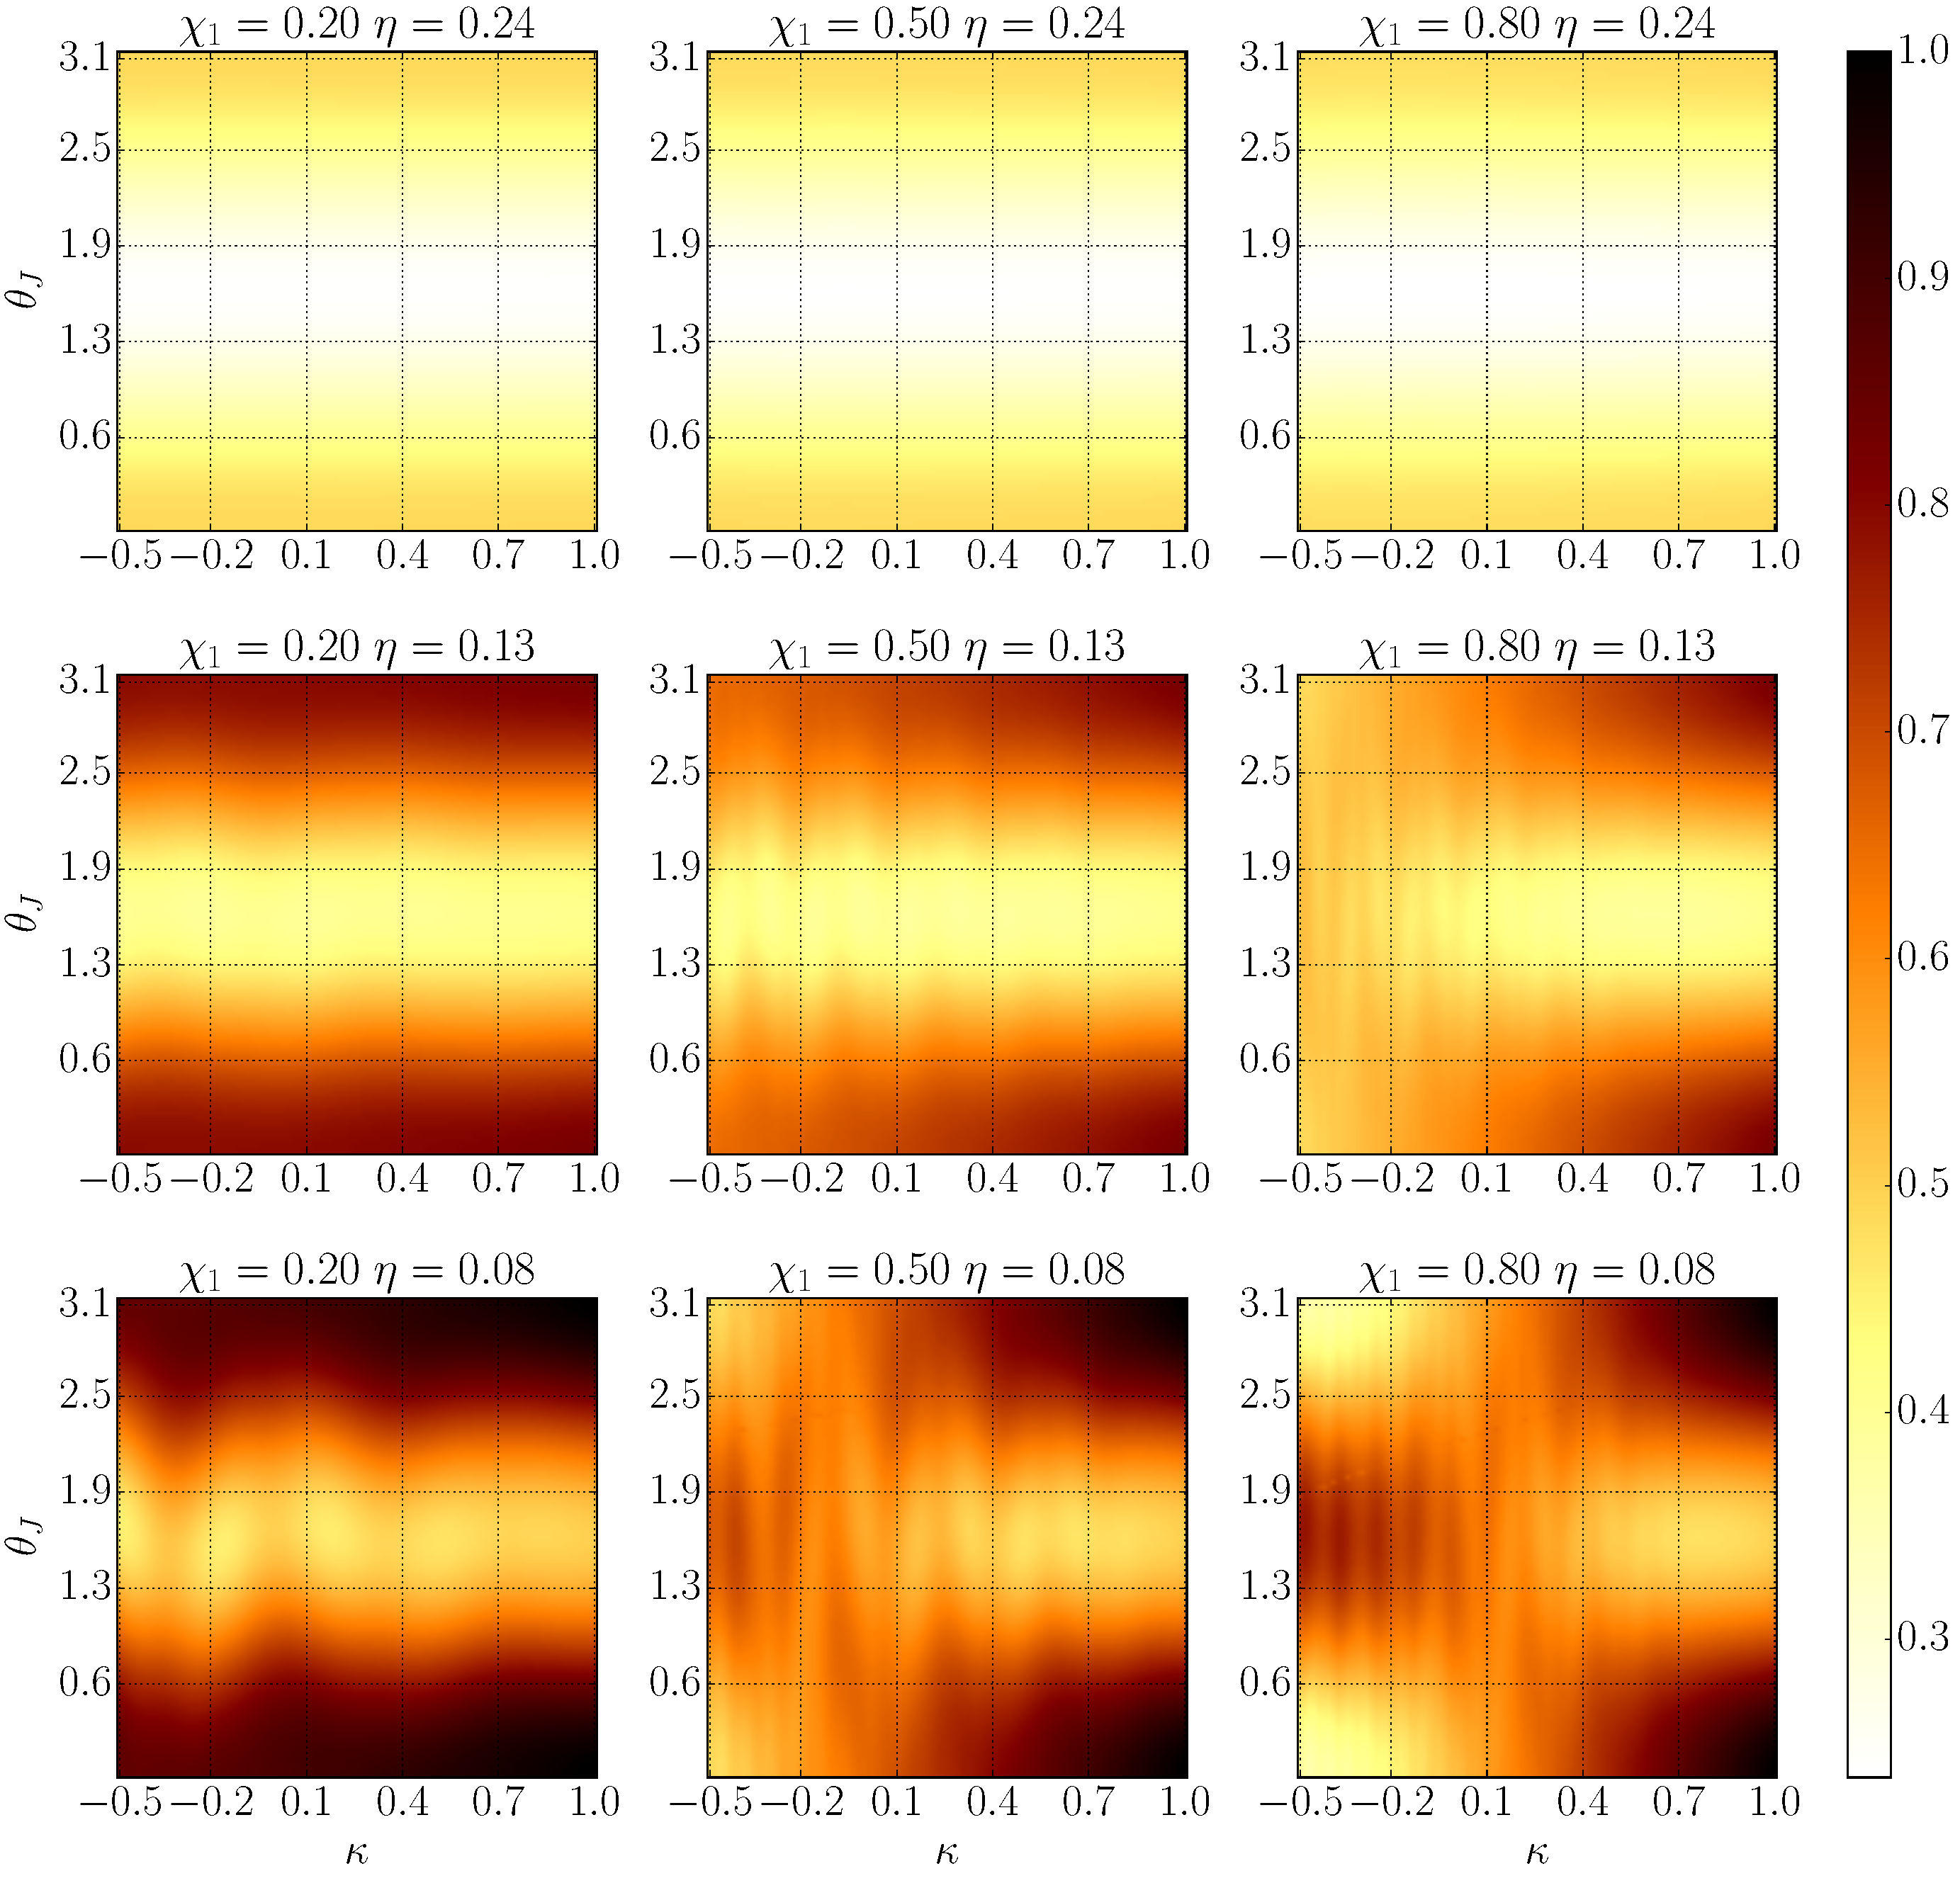
\includegraphics[width=0.7\linewidth]{figures/SNR_0F.pdf}
\caption{SNR scaled by
$\text{SNR}_{max}=20.78$. $D$ fixed to $400$ Mpc. }
\label{FIG:SNR}
\end{figure}
%===============================================================
\end{column} % END SEC II COL 3
%===============================================================
\begin{column}{.01\textwidth}\end{column} % Empty spacer column
%===========================================
\end{columns} % END SEC II
%===========================================

%===========================================
\begin{columns}[t] % BEGIN SEC III
%===========================================
\begin{column}{.01\textwidth}\end{column} % Empty spacer column
\begin{column}{.35\textwidth}
%-------------------------------------------------------------
\begin{block}{\small{Overlap Distribution of SpinTaylorF2}}
%-------------------------------------------------------------
\begin{itemize}
\item \justifying Overlap $\rightarrow~{{\cal{O}}_{m}} \equiv (h|h_m)/\sqrt{
(h|h_m) (h|h_m)}$

\vskip1ex
\item \justifying For SNR above the threshold, $m=0$ and $m=2$
are the only relevant harmonics. 

\vskip1ex
\item The $m=0$ and $m=2$ modes dominate in complimentary regions of
$(\theta_J,\, \kappa)$ space.

\begin{itemize}
\vskip1ex
\item ${\cal{O}}_{0}$ is dominant in a parabolic region symmetric about
$\theta_J=\pi/2$, in the $\kappa < 0$ region
$\rightarrow$ coverage maximum for strongly precessing systems.
\vskip1ex
\item ${\cal{O}}_{0}$ is dominant in the complimentary region where $\kappa\sim
1$, and $\theta_J = 0, \pi$ $\rightarrow$ coverage is maximum
for non-precessing systems.
\end{itemize}

\vskip1ex
\item \justifying Identified 3 regions A (${\cal{O}}_{0}\gg {\cal{O}}_{2}$),
B( ${\cal{O}}_{0}\ll {\cal{O}}_{2}$) and C (${\cal{O}}_{0}\sim {\cal{O}}_{2}$)
in the $(\theta_J, \kappa)$ space as a function of $\eta$ and $\kappa$,
associated with strongly precessing, moderately precessing and weakly/non-precessing 
systems.

\vskip1ex
\item \justifying Obtained parametric fits for the boundaries of these regions
for $(2.4\,M_\odot < m_1 < 20\,M_\odot)$, $(0 < \chi_1 < 1)$ and $(-0.5 <
\kappa < 1)$.

\vskip1ex
\begin{shaded}
\item \justifying Depending on the relative SNR contribution in the two modes,
we can put bounds on the extent of precession in the system.
\end{shaded}
\end{itemize}

\end{block}
%===============================================================
\end{column} % End of central column
%===============================================================
\begin{column}{.01\textwidth}\end{column} % Empty spacer column
\begin{column}{.59\textwidth}
%===============================================================
\begin{columns}[t]

\begin{column}{.32\textwidth}
\begin{figure}[!htb]
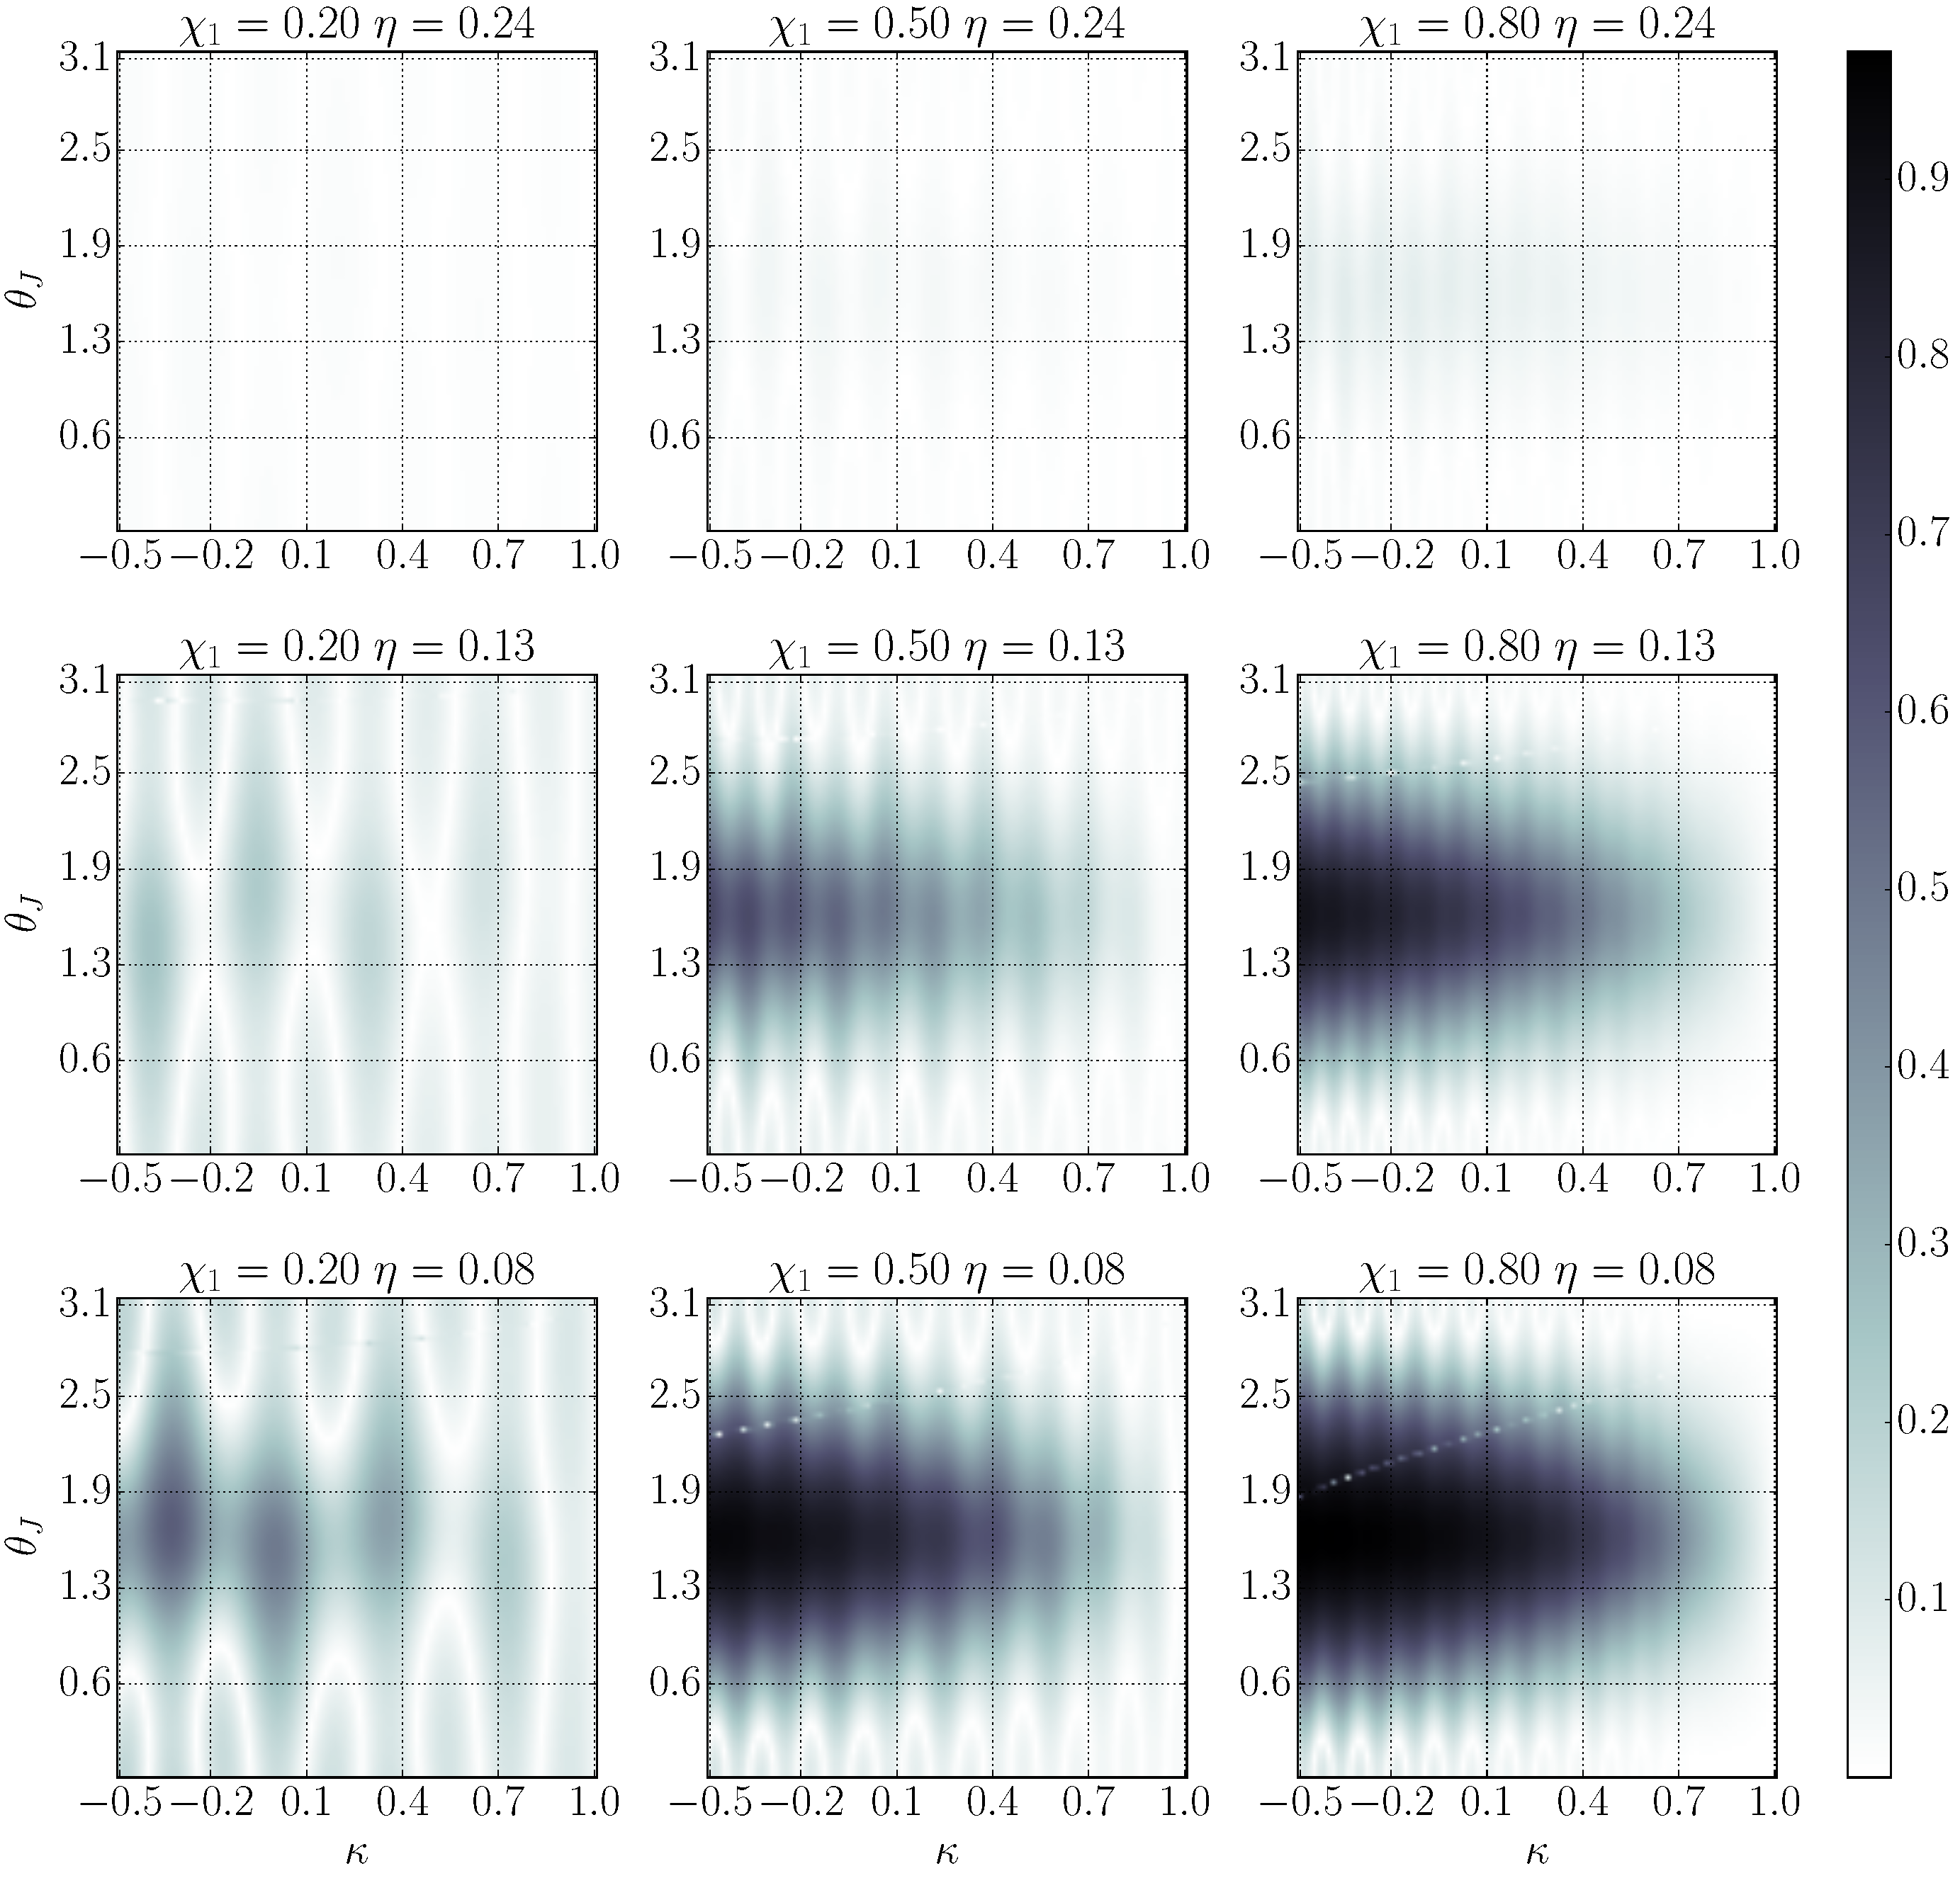
\includegraphics[width=\linewidth]{figures/OLVP_0F_P0.pdf}
\caption{${\cal{O}}_{0}$}
\label{FIG:OLVP0}
\end{figure}
\end{column}

\begin{column}{.32\textwidth}
\begin{figure}[!htb]
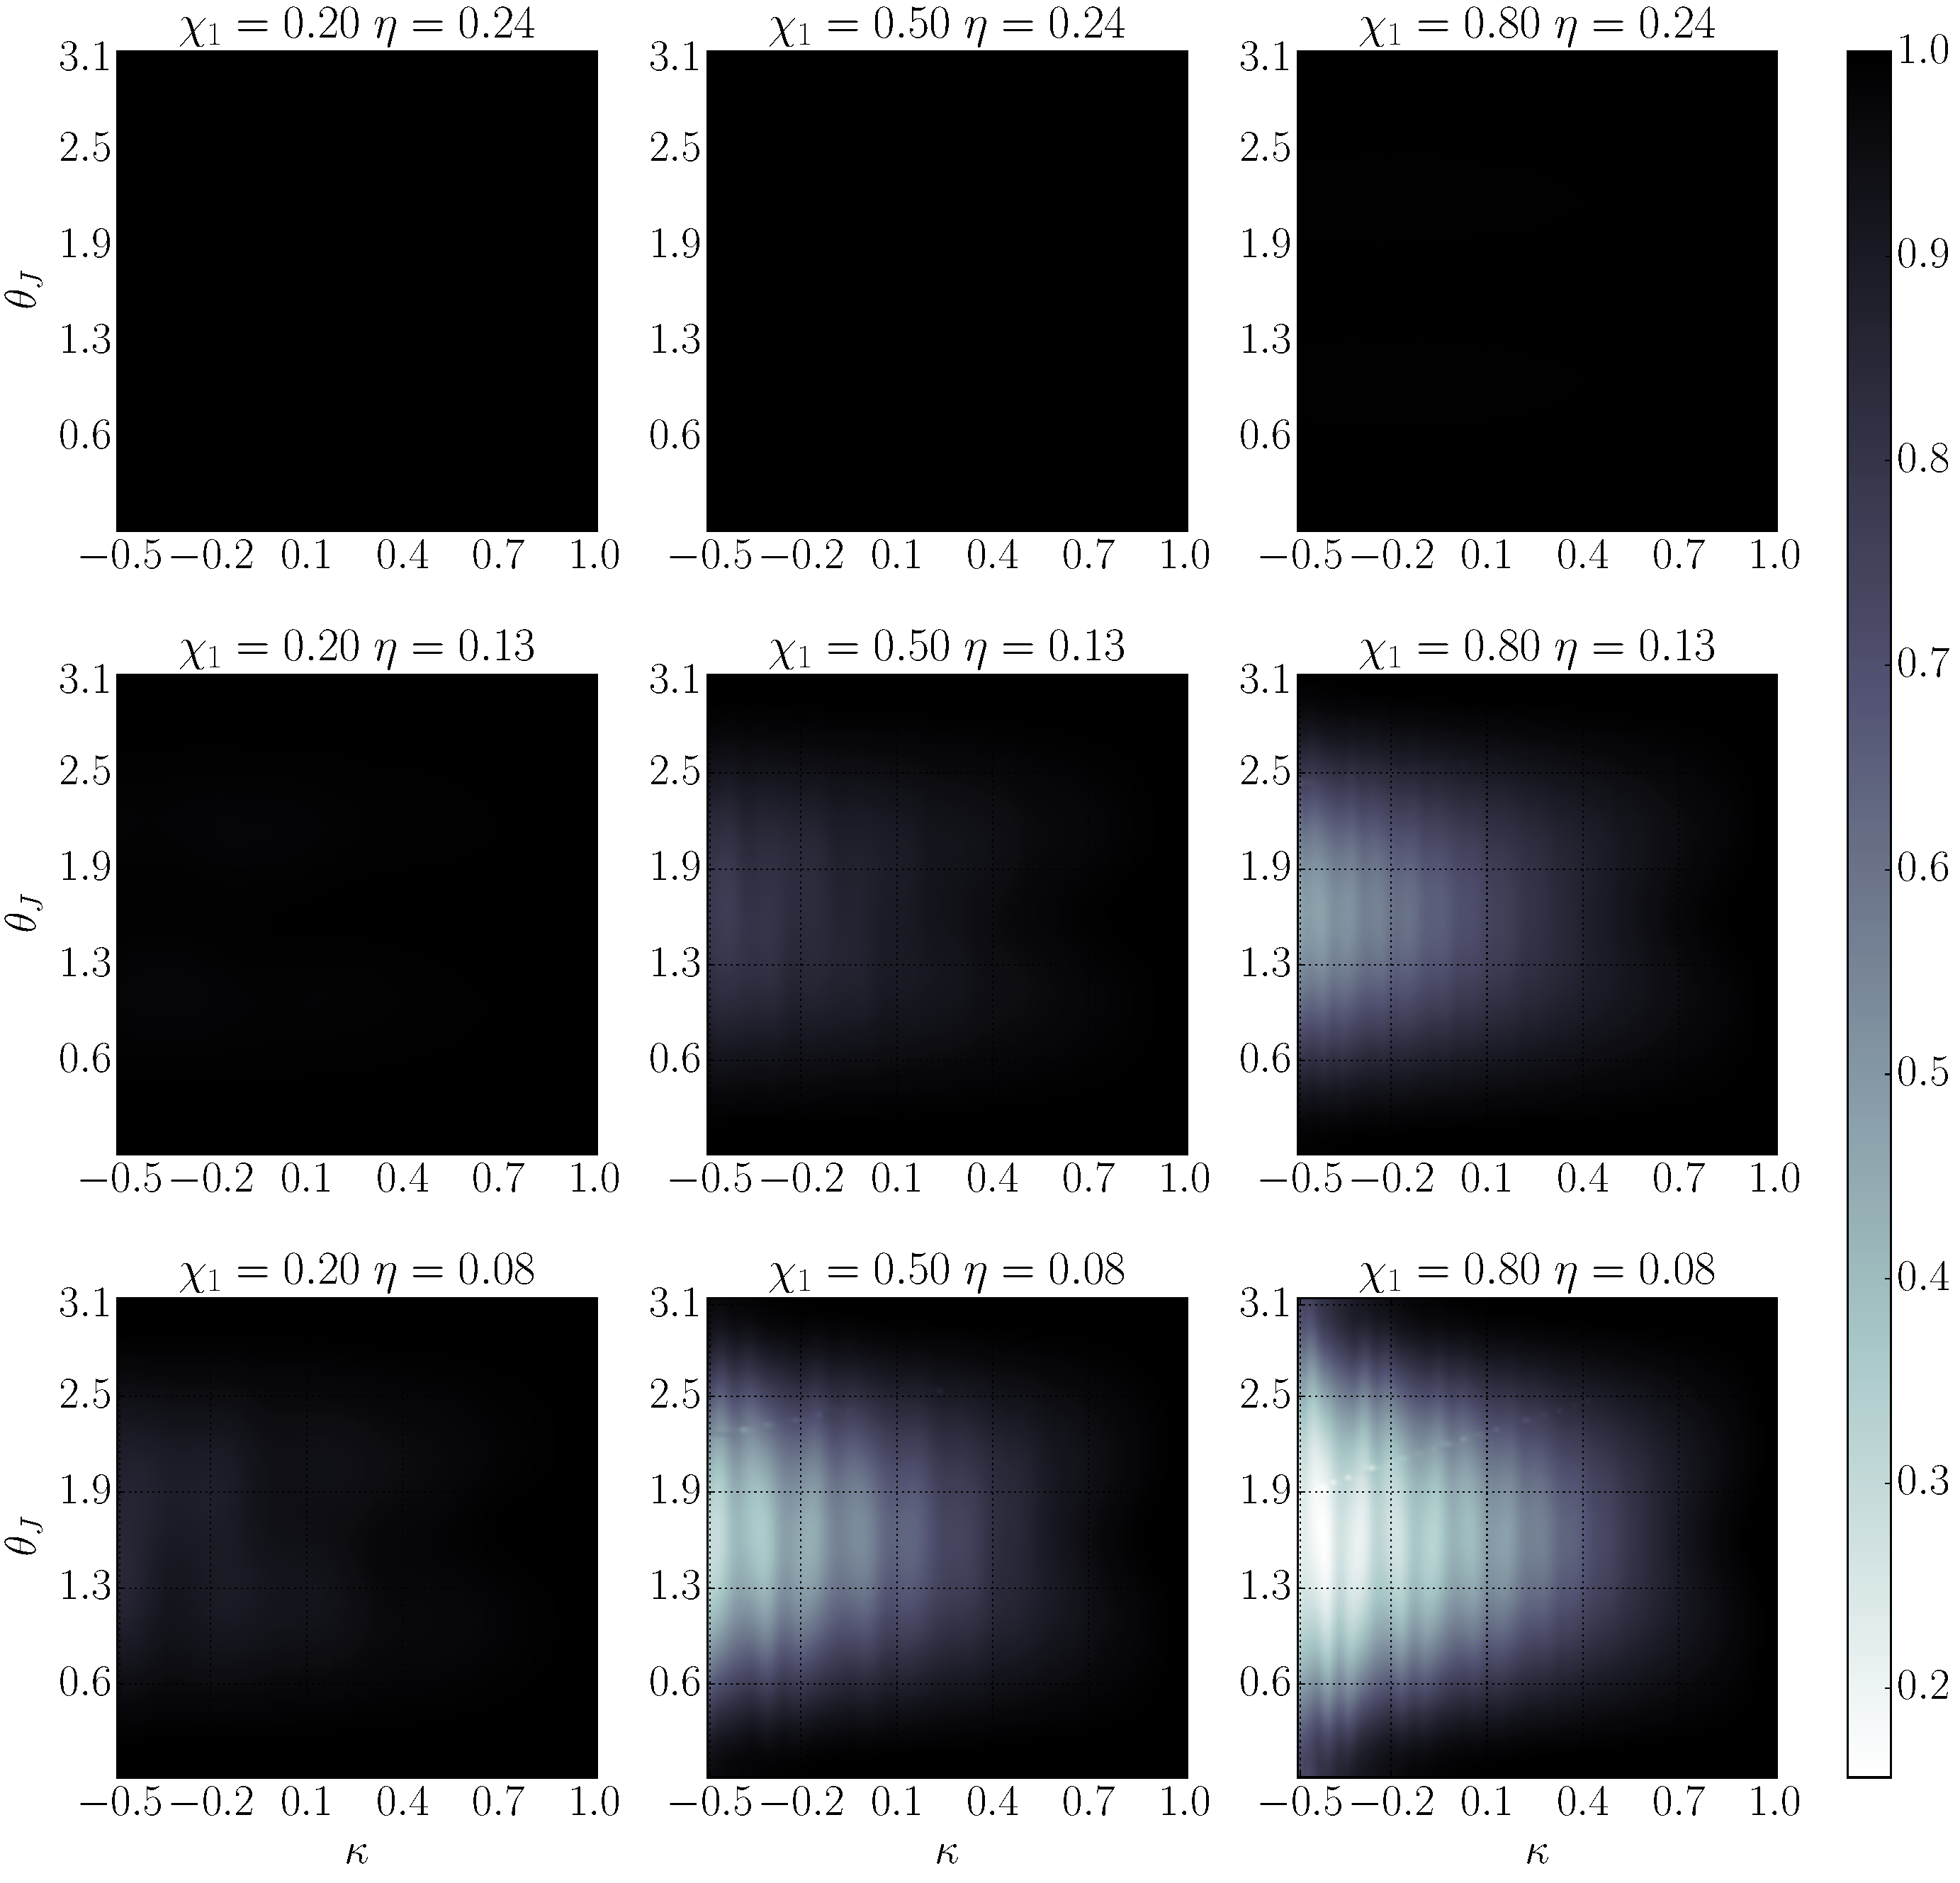
\includegraphics[width=\linewidth]{figures/OLVP_0F_P2.pdf}
\caption{${\cal{O}}_{2}$}
\label{FIG:OLVP2}
\end{figure}
\end{column}

\begin{column}{.32\textwidth}
\begin{figure}[!htb]
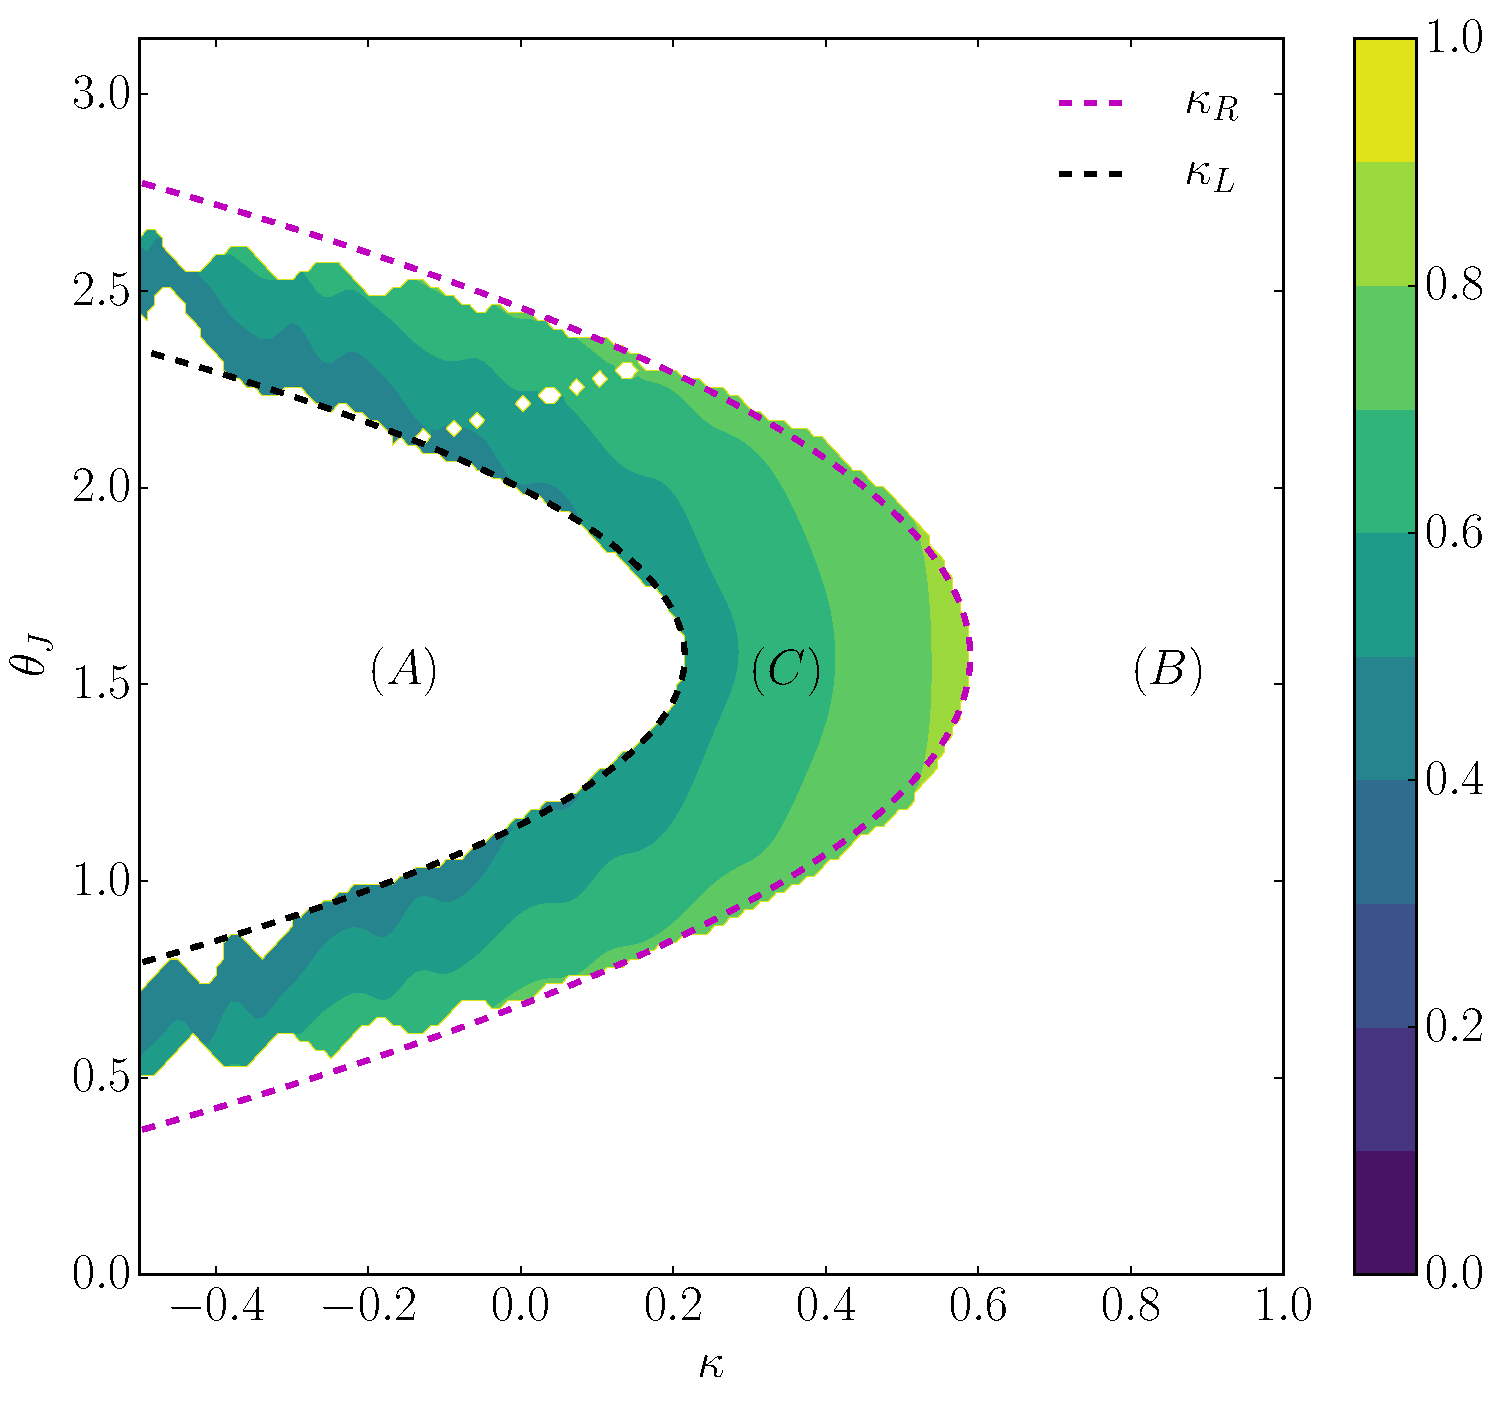
\includegraphics[width=\linewidth]{figures/OLVP_CUT.pdf}
\caption{Regions of parameter space A, B and C}.
\label{FIG:OLVPR}
\end{figure}
\end{column}

\end{columns} % END SEC III COL 2 SUBCOLS 
%===============================================================
\end{column}

\begin{column}{.01\textwidth}\end{column} % Empty spacer column
%===========================================
\end{columns} % END SEC III COLS
%===========================================

%===========================================
\begin{columns}[t] % BEGIN SEC IV
%===========================================
\begin{column}{.01\textwidth}\end{column} % Empty spacer column
%==================================================================
\begin{column}{.968\textwidth} % BEGIN CENTRAL COL
%==================================================================
%----------------------------------------------------------------------------
\begin{block}{\small{Probing astrophysical parameters of a precessing system
using information from two harmonics}}
%----------------------------------------------------------------------------
\begin{itemize}
\item \justifying Consider, if we observe a GW signal from an NSBH binary
system, and are able to determine the component masses of the system. Also,
assume that we are able to probe the SNR in the individual $m=0$ and $m=2$
spin harmonics. Then, we show below, that we can put bounds on the spin
parameters. In such a case, there are 3 possible scenarios:

\vskip1ex

\begin{description}
\item[Scenario I]: \justifying $\text{SNR}_{0} \gg {\text{SNR}}_{2}~\rightarrow$ region~A 
$\rightarrow$ strongly precessing $\rightarrow$ one can put an upper bound on
the maximum possible value of $\kappa$.
\vskip1ex
\item[Scenario II]: \justifying $\text{SNR}_{0} \sim
\text{SNR}_{2}~\rightarrow$ region~C $\rightarrow$ moderately precessing
$\rightarrow$ possible to (1)~probe the orientation parameters of the total
angular momentum vector $\mathbf{J}$ (2)~put bounds on $\kappa$.
\vskip1ex
\item[Scenario III]: \justifying $\text{SNR}_{0} \ll {\text{SNR}}_{2}~\rightarrow$ region~B 
$\rightarrow$ weakly or non-precessing system.
\end{description}
\end{itemize}

\end{block}
%===========================================
\end{column} % END CENTRAL COL
%===========================================
\begin{column}{.01\textwidth}\end{column} % Empty spacer column
%===========================================
\end{columns} % END SEC IV
%===========================================

%===========================================
\begin{columns}[t] % BEGIN SEC V COLS
%===========================================
\begin{column}{.01\textwidth}\end{column} % Empty spacer column
\begin{column}{.47\textwidth} % The first column

%---------------------------------------------
\begin{block}{\small{Scenario I : Upper bound on $\kappa$ for strongly
precessing systems}}
%---------------------------------------------
\justifying
\begin{itemize}
\item Spin modes can reveal crucial information about precession.
\item \justifying Using fits for the boundary between region~A and region~C as a
function of $\eta, \chi_1$, we obtain an upper bound on $\kappa$ as:
\begin{equation}
\kappa_{0A}(\eta, \chi_{1})~\approx  (145.83 \chi_{1} - 155.92)\, \eta^2 -
(1.10 \chi_{1} + 0.16)\, \eta+ 0.08 \, \chi_{1}+0.50,
\end{equation}
\begin{figure}[!htb]
\centering
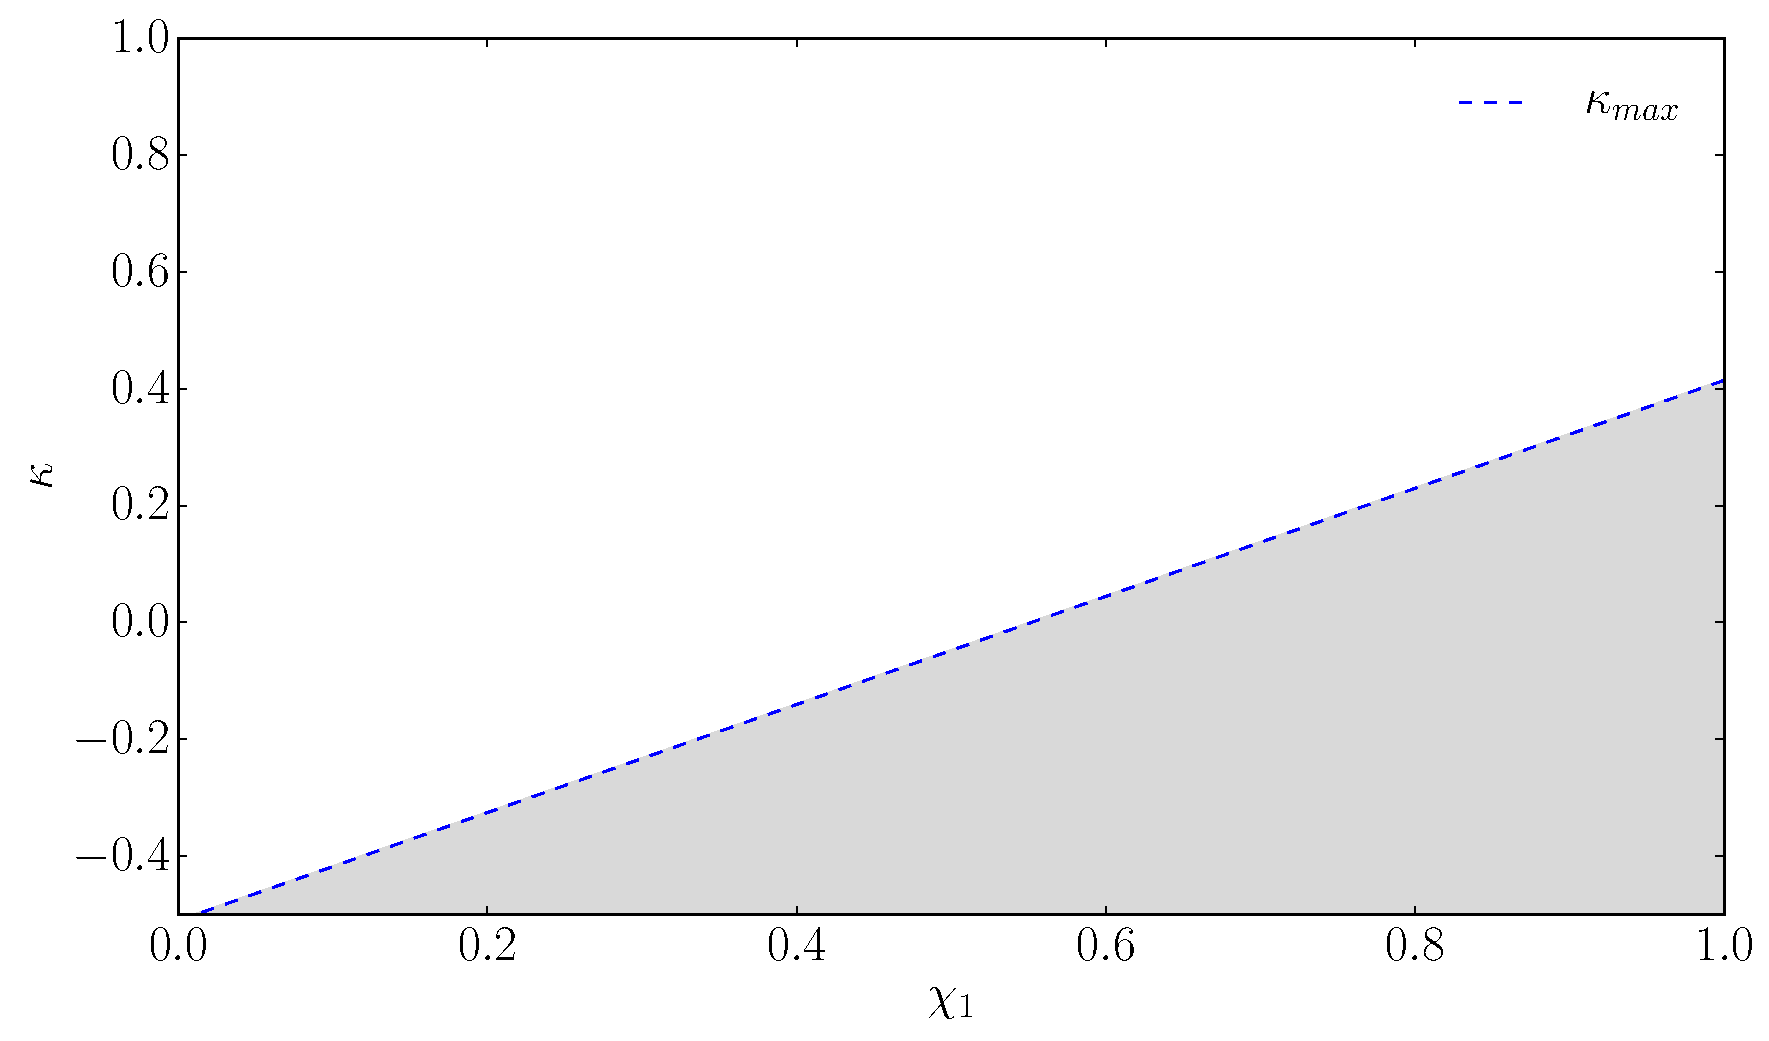
\includegraphics[width=0.7\linewidth]{figures/kappa_max_bound.pdf}
\caption{Upper bound on $\kappa$ for all possible spins; BH mass $m_1 = 14 M_{\odot}$.}
\label{FIG:KAPPA_MAX}
\end{figure}
\vskip1ex
\item Note that even for $\chi_1=1$ (highest
possible BH spin), there exists an upper bound on $\kappa \leq 0.414624$.
\end{itemize}
\end{block}

%-----------------------------------------------------------
\begin{block}{\small{Conclusions}}
%-----------------------------------------------------------
\begin{itemize}

\item \justifying Considered NSBH binary population with NS mass =
$1.4\,M_\odot$ and BH mass varying from $(2.4\,M_\odot-20\,M_\odot)$ and all
possible values of BH spins, i.e., $(0 < \chi_1 < 1)$ and spin-alignment parameter $(-0.5 < \kappa < 1)$.

\vskip1ex
\item \justifying Two dominant spin harmonics ($m = 0$ and $m = 2$) capture a large
fraction of the SNR across a large region of $(\theta_J , \kappa)$ parameter space.

\vskip1ex
\item \justifying For non-precessing as well as weakly precessing systems the
spin harmonic $m = 2$ mode contributes to most of the overlap.

\vskip1ex
\item \justifying For strongly precessing systems (highly asymmetric, high
spins and away from $\kappa= \pm 1$), the spin harmonic $m = 0$ dominates.

\vskip1ex
\item \justifying For moderately precessing systems both the harmonics
contribute.

\vskip1ex
\item \justifying Obtained parametric fits for various regions and proposed
bounds on the spin parameters
\begin{itemize}
\vskip1ex
\item \justifying Region A: $\text{SNR}_0 \gg \text{SNR}_2$, i.e, strongly
precessing systems $\rightarrow$ bound on the maximum possible value of
$\kappa$ (increases linearly with increasing $\chi_1$).

\vskip1ex
\item \justifying Region C: $\text{SNR}_0 \sim \text{SNR}_2$, i.e, moderately
precessing systems $\rightarrow$ also gives bound on the maximum possible
value of $\kappa$.
\end{itemize}

\vskip1ex
\item[] \justifying This clearly shows that for moderately precessing systems,
the value of the upper bound on $\kappa$ is higher than that of the highly
precessing case for same value of BH spin  ($\kappa \leq 0.414624$ for
strongly precessing case, whereas $\kappa \leq 0.64984$ for moderately
precessing cases.)

\vskip1ex
\item \justifying Using $\text{SNR}_0, \text{SNR}_2$, the orientation of total
angular momentum vector can be probed.

\end{itemize}
\end{block}
\end{column}

\begin{column}{.005\textwidth}\end{column} % Empty spacer column
\begin{column}{.47\textwidth} % The second column

%---------------------------------------------
\begin{block}{\small{Scenario II : Upper bound on $\kappa$ for moderately
precessing systems}}
%---------------------------------------------
\justifying
\begin{itemize}
\item \justifying Similar to Scenario I, we use fits for the boundary between region~C and region~B as a
function of $\eta, \chi_1$, to obtain an upper bound on $\kappa$ as:
\begin{equation}
\kappa_{0B}(\eta, \chi_{1})~\approx (48.98\chi_{1} - 57.13) \,\eta^2 +
(1.96{\chi_{1}}-2.39)\, \eta - 0.09 \, \chi_{1} +0.82,
\end{equation}
\begin{figure}[!htb]
\centering
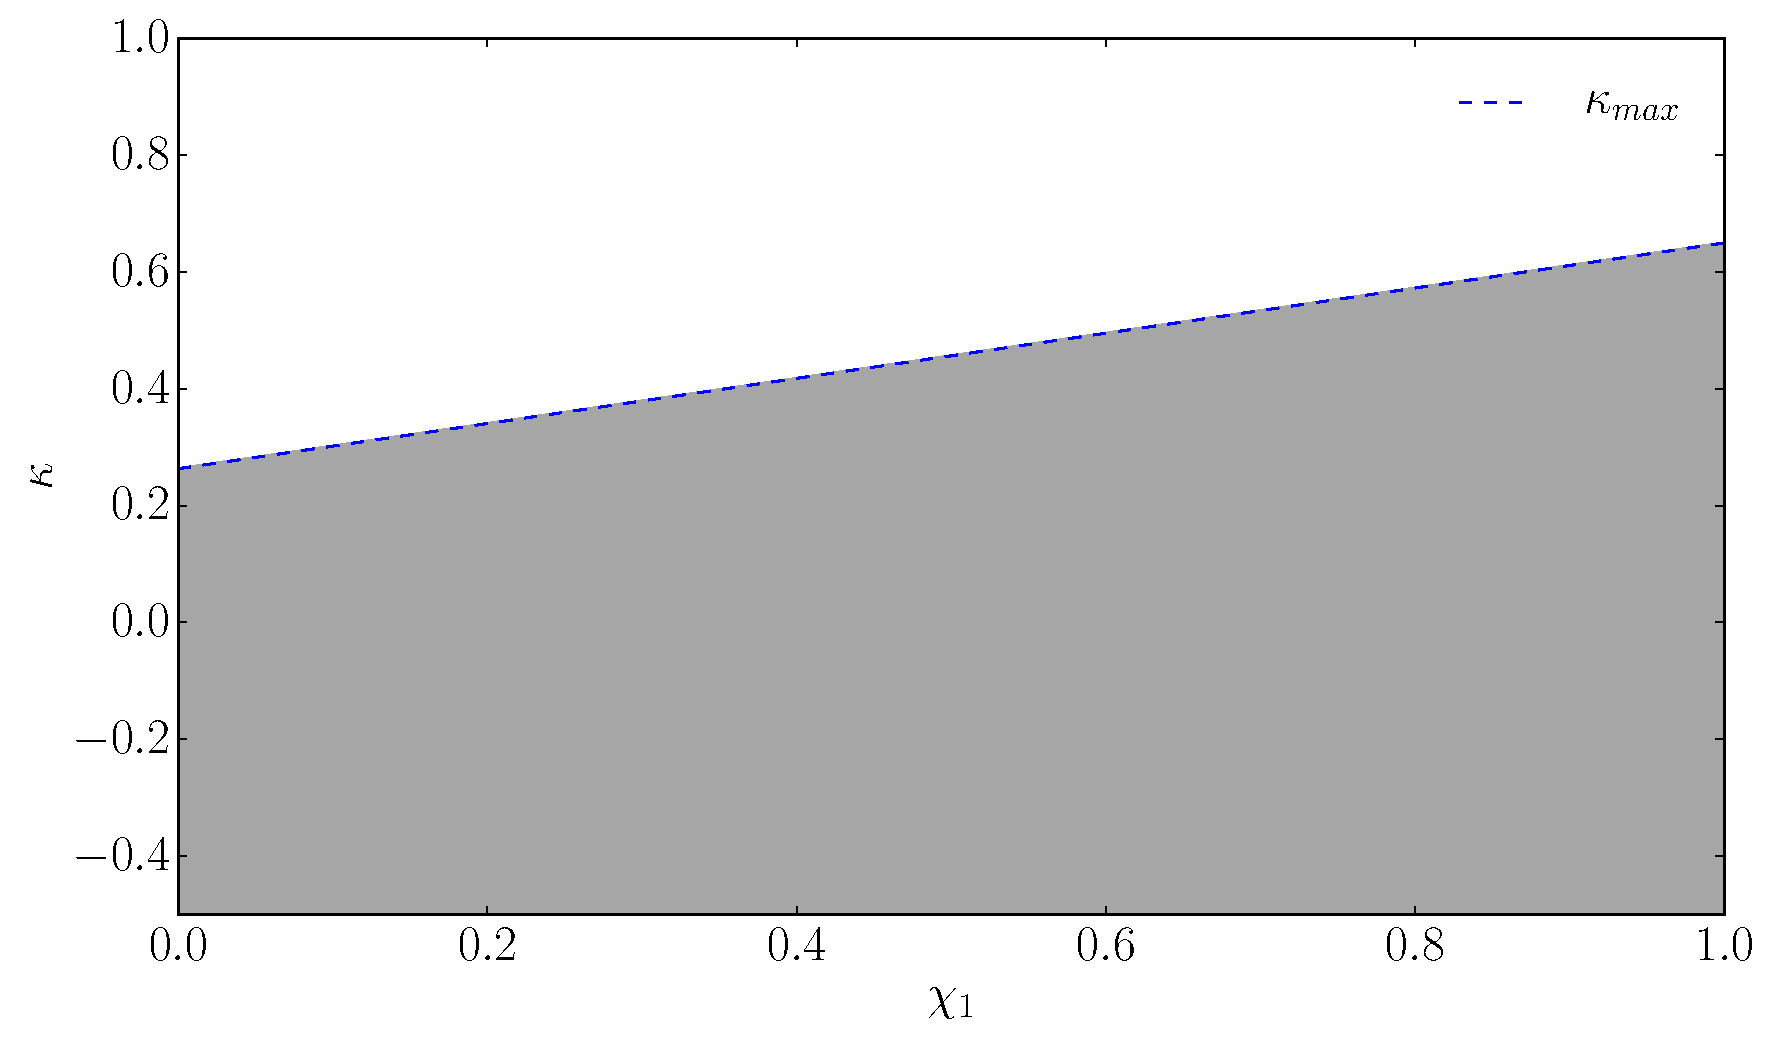
\includegraphics[width=0.7\linewidth]{figures/kappa_max_bound_S2.pdf}
\caption{Upper bound on $\kappa$ for all possible spins; BH mass $m_1 = 14 M_{\odot}$ for moderately precessing systems.}
\label{FIG:KAPPA_MAX}
\end{figure}
\vskip1ex
\item Even for moderately precessing systems $\kappa \leq 0.64984$ for $\chi_1=1$.
\vskip2.3ex
\end{itemize}
\end{block}


%------------------------------------------------------------------------------------------------------
\begin{block}{\small{Scenario II : Estimation of angular parameters $~\theta_J$ and $\psi_J$}}
%------------------------------------------------------------------------------------------------------
\justifying
\begin{itemize}
\item Given $(\text{SNR}_2, \text{SNR}_0)~\Rightarrow$ $\hat{H}_0, \hat{H}_2$
(maximum likelihood estimates)
\vskip1ex
\item \justifying Then, using the amplitude estimates $H_0$ and $H_2$, along
with the phase difference $\phi_2 - \phi_0$ of the two spin harmonics, we can
estimate $\hat{\theta}_J, \hat{\psi'}_J$:
\begin{align}
\begin{split}
\cos\hat{\theta}_J =& \left(\frac{3\hat{H}_2~ \cos(\phi_2-\phi_0)-2 \hat{H}_0}{3\hat{H}_2~
\cos(\phi_2-\phi_0)+2 \hat{H}_0}\right)^{1/2}, \\
\cos 2\,\hat{\psi}'_J =& -\sin (\phi_2-\phi_0)/ \cos(\theta_J), 
\label{theta_J}
\end{split}
\end{align}
where $\hat{\theta}_J, \hat{\psi'}_J$ define the orientation of the total angular momentum vector $\mathbf{J}$.
\end{itemize}
\end{block}

%------------------------------------------------------------------------------------------------------
\begin{block}{\small{Acknowledgments}}
%------------------------------------------------------------------------------------------------------
\justifying
\begin{itemize}
\item Kumar Atmjeet is supported by the DST-MPG Max Planck Partner Group fund at IISER
TVM and the CCMS fund of IISER TVM. \'E Chassande-Mottin acknowledges the
support from CNRS, PICS grant respectively. 
\vskip1ex
\item[] \justifying This document has a LIGO document number LIGO-G1700374.
\end{itemize}
\end{block}

%-----------------------------------------------------------
\begin{block}{\small{References}}
%-----------------------------------------------------------
\begin{itemize}
\item A. Lundgren and R. O’Shaughnessy, Phys. Rev. D \textbf{89}, 044021 (2014), 1304.3332.
\end{itemize}

\end{block}

\end{column} % End of the second column
\begin{column}{.01\textwidth}\end{column} % Empty spacer column
%===========================================
\end{columns} % END SEC 5 COLS
%===========================================

%=======================================
\end{frame} % End of the enclosing frame
%========================================================================================
\end{document}
%========================================================================================